\section{Written Description and Diagrams of Circuit}
\subsection{Written Description of Galaga}
\quad
This project is essentially the 1981 fixed shooter arcade Galaga game (the specific mechanics for which can be easily found online).
In it's current iteration, only one type of animating enemy is displayed.
The player ship can be controlled via a joystick shield and bullets can be shot with the A button on the shield.
Key 0 is assigned as a global reset for the project.
Hit detection for the bullet is implemented such that shooting an enemy makes it despawn.
While only one type of enemy is present, the sprite ROM includes multiple types of enemies.
Thus, due to the modular design, multiple types of enemies can be easily displayed.

\subsection{Block Diagram}
\begin{figure}[!htb]
  \centering
  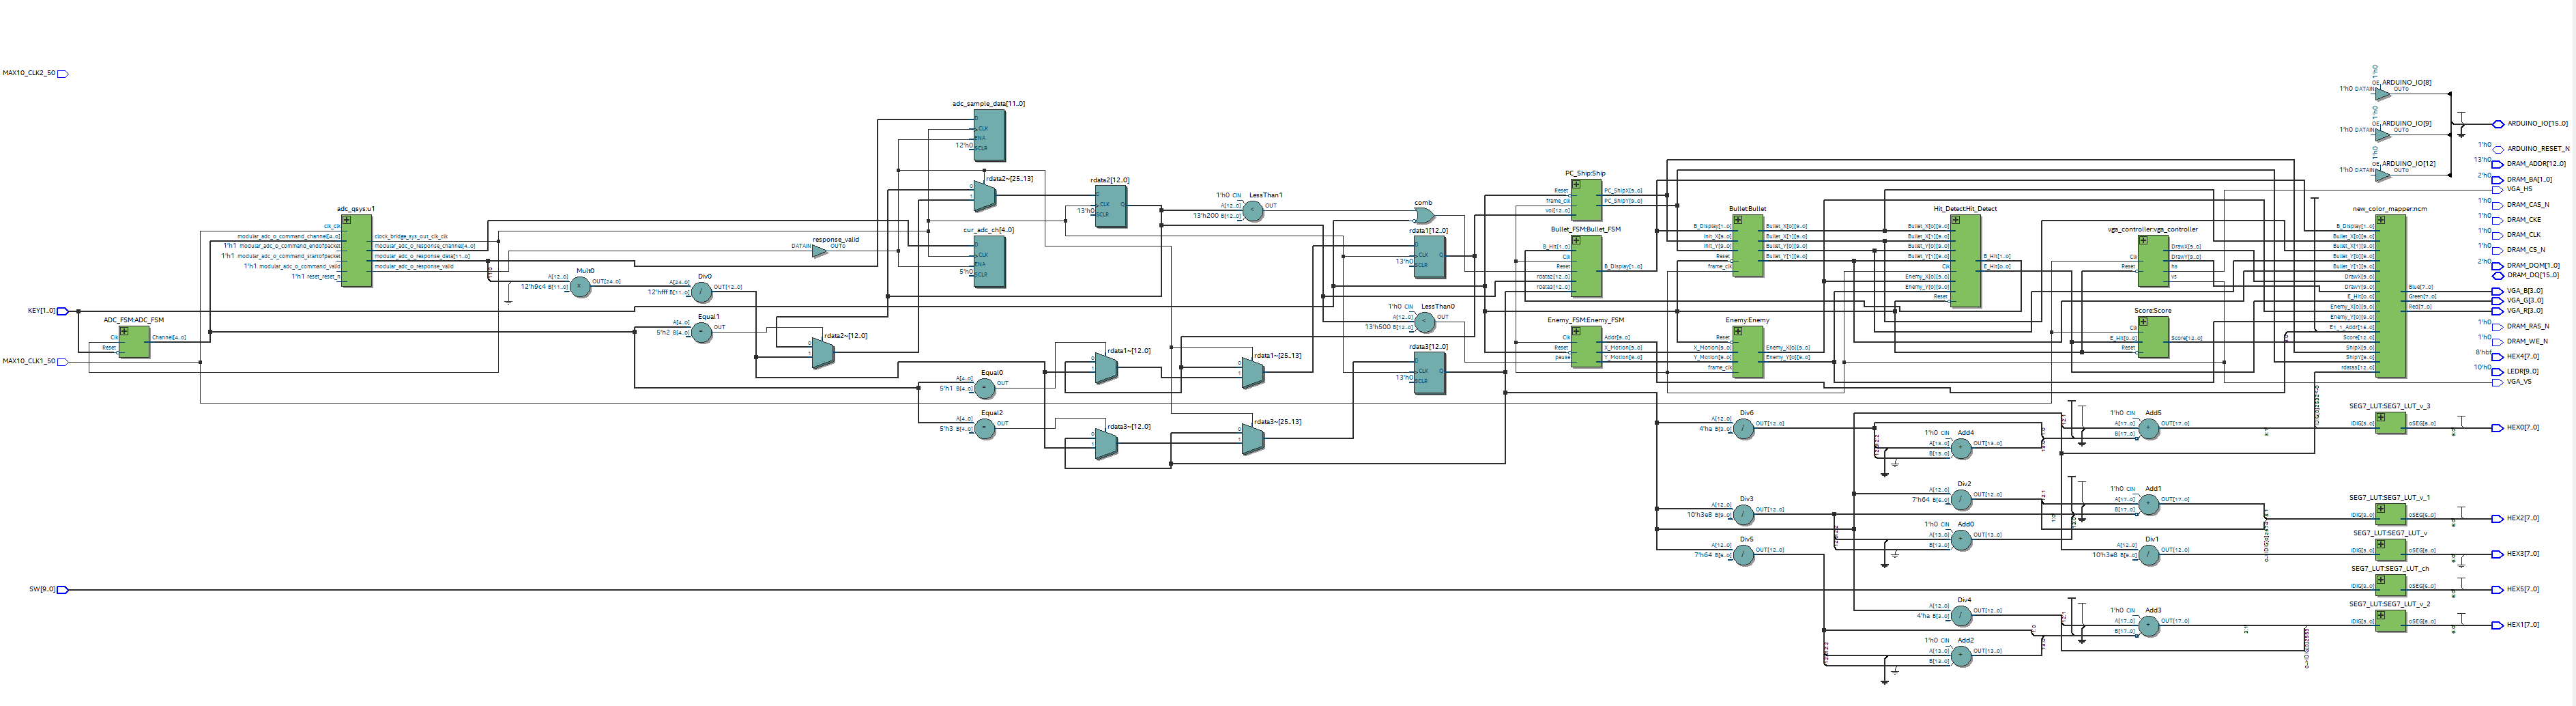
\includegraphics[width=\linewidth]{rtl.png}
  \caption{Top Level RTL Diagram}
  \label{Fig: TLRTL}
\end{figure}

\pagebreak


\subsection{State Diagram}
\quad
There are multiple FSMs in this project.
One of the more interesting ones have been included below.

\begin{figure}[!htb]
  \centering
  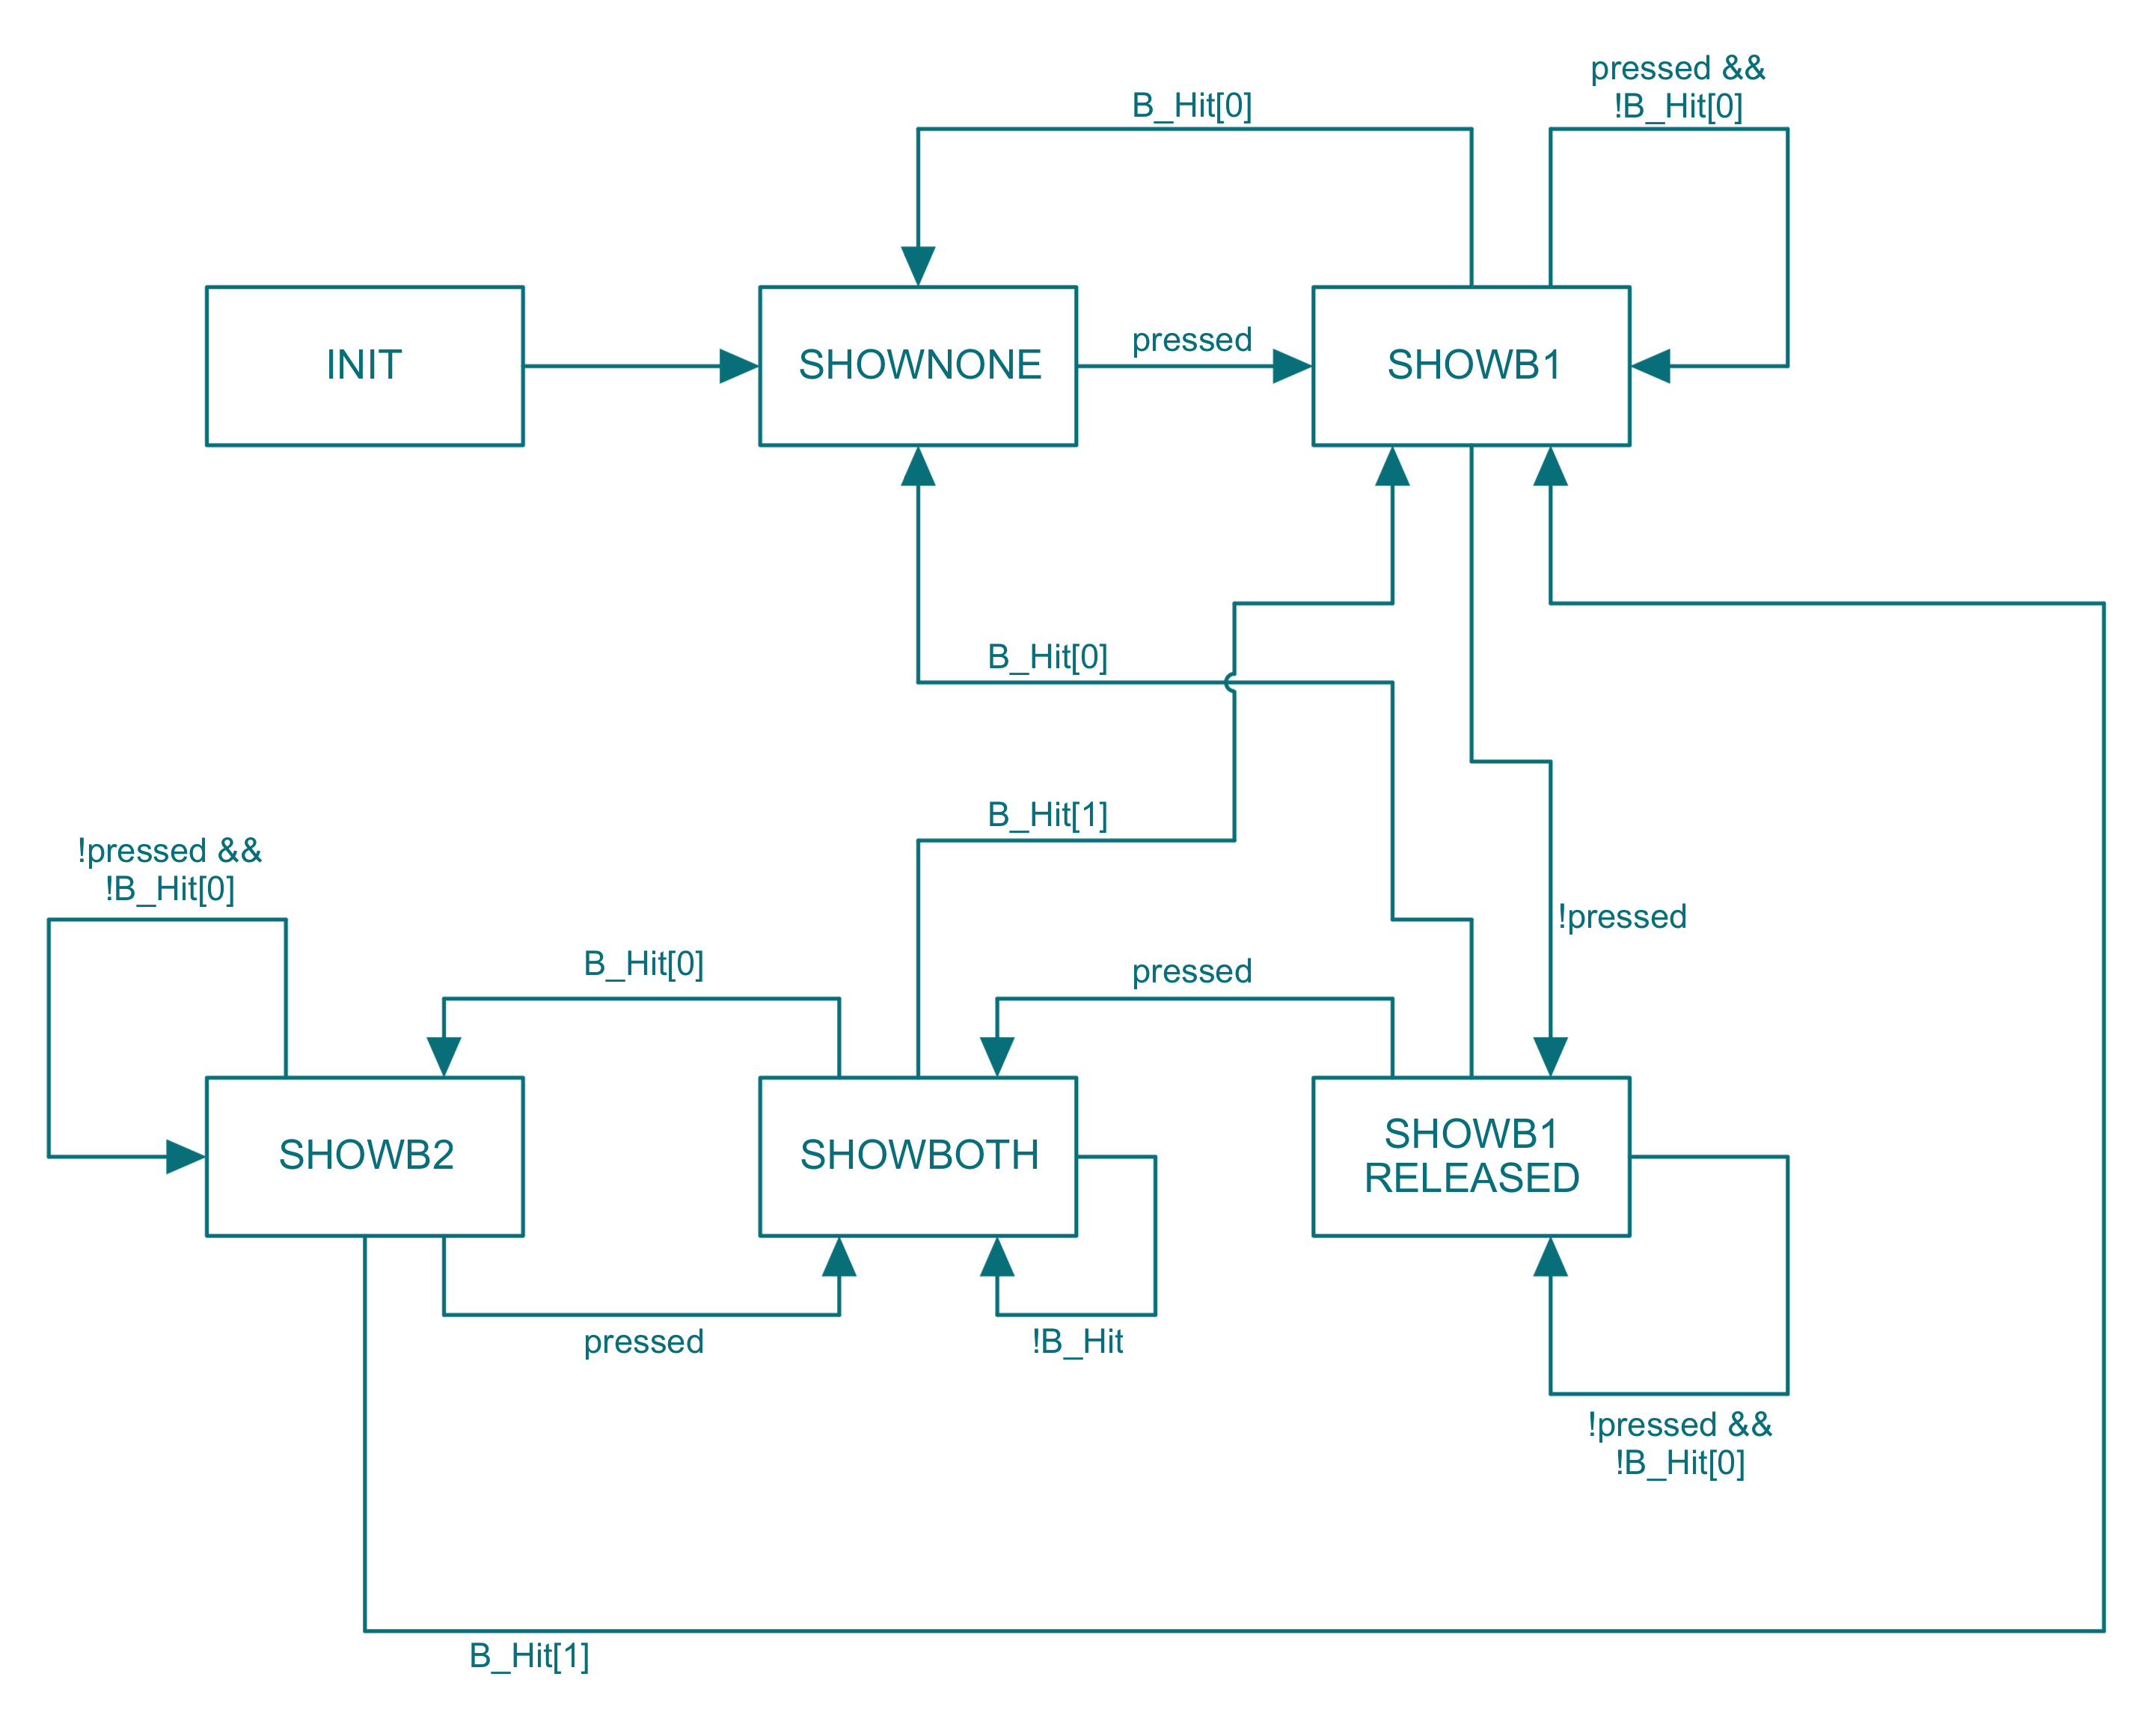
\includegraphics[width=\linewidth]{bullet_fsm.png}
  \caption{Bullet FSM}
  \label{Fig: BulletFSM}
\end{figure}

